% ============================================================
%  Relazione Accademica — Modello SIR come Catena di Markov
%  Autore  : Francesco Castaldi
%  Corso   : Modelli Probabilistici — Università di Bologna
%  Docente : Prof. Salvatore Federico
%  A.A.    : 2025/2026
% ============================================================

\documentclass[11pt, a4paper]{article}

% ── Encoding & lingua ──────────────────────────────────────
\usepackage[utf8]{inputenc}
\usepackage[T1]{fontenc}
\usepackage[italian]{babel}

% ── Impaginazione ──────────────────────────────────────────
\usepackage[
  top=2.5cm, bottom=2.5cm,
  left=3cm,  right=3cm
]{geometry}
\usepackage{microtype}
\usepackage{setspace}
\onehalfspacing

% ── Matematica ────────────────────────────────────────────
\usepackage{amsmath, amssymb, amsthm}
\usepackage{mathtools}

% Ambienti teorema
\theoremstyle{plain}
\newtheorem{theorem}{Teorema}[section]
\newtheorem{proposition}[theorem]{Proposizione}
\newtheorem{lemma}[theorem]{Lemma}
\theoremstyle{definition}
\newtheorem{definition}[theorem]{Definizione}
\newtheorem{example}[theorem]{Esempio}
\theoremstyle{remark}
\newtheorem{remark}[theorem]{Osservazione}

% ── Tabelle & figure ──────────────────────────────────────
\usepackage{booktabs}
\usepackage{graphicx}
\usepackage{float}
\usepackage{caption}
\captionsetup{font=small, labelfont=bf}

% ── Codice sorgente ───────────────────────────────────────
\usepackage{listings}
\usepackage{xcolor}

\definecolor{codegreen}{rgb}{0,0.5,0}
\definecolor{codegray}{rgb}{0.5,0.5,0.5}
\definecolor{codeblue}{rgb}{0,0,0.7}
\definecolor{backcolour}{rgb}{0.97,0.97,0.97}

\lstdefinestyle{pythonstyle}{
  backgroundcolor=\color{backcolour},
  commentstyle=\color{codegreen}\itshape,
  keywordstyle=\color{codeblue}\bfseries,
  numberstyle=\tiny\color{codegray},
  stringstyle=\color{orange!70!black},
  basicstyle=\ttfamily\small,
  breakatwhitespace=false,
  breaklines=true,
  captionpos=b,
  numbers=left,
  numbersep=5pt,
  showspaces=false,
  showstringspaces=false,
  tabsize=4,
  language=Python,
  frame=single,
  rulecolor=\color{gray!30},
}
\lstset{style=pythonstyle}

% ── Hyperlink ──────────────────────────────────────────────
\usepackage[
  colorlinks=true,
  linkcolor=black,
  citecolor=black,
  urlcolor=blue!70!black
]{hyperref}

% ── Intestazioni ──────────────────────────────────────────
\usepackage{fancyhdr}
\pagestyle{fancy}
\fancyhf{}
\fancyhead[L]{\small Modello SIR come Catena di Markov}
\fancyhead[R]{\small F.\ Castaldi — A.A.\ 2025/2026}
\fancyfoot[C]{\thepage}
\renewcommand{\headrulewidth}{0.4pt}

% ── Utilità ───────────────────────────────────────────────
\usepackage{enumitem}
\usepackage{bm}
\newcommand{\E}{\mathbb{E}}
\newcommand{\Prob}{\mathbb{P}}
\newcommand{\N}{\mathbb{N}}
\newcommand{\R}{\mathbb{R}}
\newcommand{\uno}{\mathbf{1}}

% ═══════════════════════════════════════════════════════════
\begin{document}
% ═══════════════════════════════════════════════════════════

% ── Frontespizio ──────────────────────────────────────────
\begin{titlepage}
  \centering
  \vspace*{2cm}
  {\Large\bfseries Alma Mater Studiorum — Università di Bologna}\\[0.4cm]
  {\large Dipartimento di Matematica}\\[0.3cm]
  {\large Corso di Laurea in Informatica}\\[2cm]

  \rule{\linewidth}{0.5pt}\\[0.4cm]
  {\LARGE\bfseries Simulazione di un modello epidemiologico SIR}\\[0.3cm]
  {\LARGE\bfseries come catena di Markov a tempo discreto}\\[0.4cm]
  \rule{\linewidth}{0.5pt}\\[2cm]

  \begin{minipage}{0.48\textwidth}
    \begin{flushleft}
      \textbf{Docente}\\
      Prof.\ Salvatore Federico\\[0.3cm]
      \textbf{Corso}\\
      Metodi Probabilistici per le Applicazioni\\
      Modelli Probabilistici (518512)
    \end{flushleft}
  \end{minipage}
  \hfill
  \begin{minipage}{0.48\textwidth}
    \begin{flushright}
      \textbf{Studente}\\
      Francesco Castaldi\\[0.3cm]
      \textbf{Anno Accademico}\\
      2025/2026
    \end{flushright}
  \end{minipage}

  \vfill
  {\large Appello: Prima settimana di Settembre 2026}
\end{titlepage}

% ── Indice ────────────────────────────────────────────────
\tableofcontents
\newpage

% ═══════════════════════════════════════════════════════════
\section*{Abstract}
\addcontentsline{toc}{section}{Abstract}
% ═══════════════════════════════════════════════════════════

Il presente lavoro studia un modello epidemiologico di tipo SIR (Suscettibili–Infetti–Rimossi) su
una popolazione finita di $N = 100$ individui, formalizzandolo rigorosamente come una
\emph{catena di Markov a tempo discreto}. L'obiettivo non è produrre una previsione epidemiologica
realistica, bensì applicare i risultati fondamentali della teoria delle catene di Markov —
proprietà di Markov, matrice di transizione, classificazione degli stati, assorbimento —
a un caso concreto e numericamente trattabile.

Dopo aver definito lo spazio degli stati e derivato le probabilità di transizione a partire da
meccanismi binomiali indipendenti, si verifica che il processo soddisfa la proprietà di Markov
e se ne classificano gli stati (assorbenti vs.\ transitori). Per popolazioni di taglia realistica,
il comportamento globale viene esplorato mediante simulazione Monte Carlo ($M = 1000$
replicazioni, seed fisso per riproducibilità). I risultati quantitativi — picco medio degli infetti
$\approx 21.9$, tempo medio di estinzione $\approx 86.7$ passi, rimossi finali $\approx 76.6$ —
vengono confrontati con la soluzione deterministica delle equazioni differenziali di
Kermack--McKendrick, evidenziando l'apporto aggiuntivo di informazione della trattazione
stocastica.

\bigskip
\noindent\textbf{Parole chiave:} catene di Markov, modello SIR, simulazione Monte Carlo,
stati assorbenti, limite fluido.

\newpage

% ═══════════════════════════════════════════════════════════
\section{Introduzione}
% ═══════════════════════════════════════════════════════════

La propagazione di una malattia infettiva in una popolazione finita è un fenomeno
intrinsecamente stocastico: l'incontro tra un suscettibile e un infetto è un evento casuale,
la guarigione avviene con una certa probabilità indipendente per ciascun individuo.
Un modello deterministico — come le classiche equazioni di Kermack--McKendrick~\cite{kermack1927} —
cattura l'andamento medio, ma ignora la variabilità campionaria e, soprattutto, non distingue
tra popolazioni di taglia diversa.

Formalizzare il processo SIR come \emph{catena di Markov a tempo discreto} permette di collocare
il problema nel quadro rigoroso della teoria probabilistica e di rispondere a domande quali:
\emph{con quale probabilità l'epidemia si estingue in meno di $T$ passi? Qual è il numero atteso
di individui mai infettati?} Queste domande non hanno una risposta esatta nel framework
deterministico, ma sono naturalmente formulabili nello spazio degli stati markoviano.

Il lavoro ha una finalità dichiaratamente didattica: ogni scelta modellistica è orientata a
mettere in luce la struttura probabilistica del sistema, sacrificando dettagli di realismo
biologico (eterogeneità della popolazione, dinamiche demografiche, struttura di contatto
non omogenea) che esulano dall'obiettivo formativo.

\subsection{Organizzazione del documento}

La \autoref{sec:modello} introduce il modello SIR e ne deriva la struttura markoviana.
La \autoref{sec:esempio} illustra con $N=3$ la costruzione esplicita della matrice di
transizione. La \autoref{sec:simulazione} descrive l'algoritmo di simulazione Monte Carlo.
La \autoref{sec:risultati} riporta i risultati numerici. La \autoref{sec:teoria} sviluppa
l'analisi teorica della catena (classificazione degli stati, assorbimento, tempo medio).
La \autoref{sec:limitefluido} confronta il modello stocastico con l'approssimazione ODE.
La \autoref{sec:conclusioni} trae le conclusioni didattiche.

% ═══════════════════════════════════════════════════════════
\section{Modello SIR come catena di Markov}
\label{sec:modello}
% ═══════════════════════════════════════════════════════════

\subsection{Definizione dello spazio degli stati}

Si considera una popolazione \emph{chiusa} di dimensione costante $N \in \N$, $N \geq 1$.
In ogni istante discreto $t \in \N_0 = \{0, 1, 2, \ldots\}$ lo stato del sistema è descritto
dalla tripla

\[
  X_t = (S_t,\, I_t,\, R_t),
\]

dove $S_t, I_t, R_t \in \N_0$ denotano rispettivamente il numero di
\emph{Suscettibili}, \emph{Infetti} e \emph{Rimossi} (individui guariti e
immunizzati) al tempo $t$. Il vincolo di conservazione

\begin{equation}\label{eq:conservazione}
  S_t + I_t + R_t = N \qquad \forall\, t \in \N_0
\end{equation}

implica che basta specificare $(S_t, I_t)$ per determinare $R_t = N - S_t - I_t$.
Lo \emph{spazio degli stati} è pertanto l'insieme finito

\begin{equation}\label{eq:spazio_stati}
  E = \bigl\{(s,i,r) \in \N_0^3 : s + i + r = N\bigr\},
\end{equation}

la cui cardinalità è

\[
  |E| = \binom{N+2}{2} = \frac{(N+1)(N+2)}{2}.
\]

Per $N = 100$ si ottengono $|E| = 5151$ stati distinti.

\subsection{Probabilità di transizione e proprietà di Markov}

La dinamica temporale è governata da due meccanismi \emph{stocastici e indipendenti}
che operano in ciascun passo temporale:

\begin{itemize}[leftmargin=2em]
  \item \textbf{Contagio:} ogni suscettibile viene infettato con probabilità
    $p_{\mathrm{SI}} = \beta\, I_t / N$, indipendentemente dagli altri.
    Il numero di nuovi contagi è quindi
    \[
      C_t \mid (S_t = s, I_t = i) \;\sim\; \mathrm{Bin}\!\left(s,\; \frac{\beta\, i}{N}\right).
    \]

  \item \textbf{Guarigione:} ogni infetto guarisce con probabilità $\gamma$,
    indipendentemente dagli altri e dagli eventi di contagio.
    Il numero di guarigioni è
    \[
      G_t \mid I_t = i \;\sim\; \mathrm{Bin}(i,\, \gamma).
    \]
\end{itemize}

Lo stato si aggiorna secondo

\begin{equation}\label{eq:aggiornamento}
  \begin{aligned}
    S_{t+1} &= S_t - C_t,\\
    I_{t+1} &= I_t + C_t - G_t,\\
    R_{t+1} &= R_t + G_t.
  \end{aligned}
\end{equation}

\begin{proposition}[Proprietà di Markov]
  Il processo $\{X_t\}_{t \geq 0}$ è una catena di Markov omogenea su $E$.
\end{proposition}

\begin{proof}
  La distribuzione di $(C_t, G_t)$ — e quindi di $X_{t+1}$ —
  dipende dalla storia del processo \emph{esclusivamente} attraverso lo stato corrente
  $(S_t, I_t, R_t)$: le Binomiali hanno parametri che dipendono solo da $s = S_t$ e $i = I_t$.
  Formalmente, per ogni $(s', i', r') \in E$ e ogni storia
  $(x_0, \ldots, x_{t-1}) \in E^t$,

  \[
    \Prob\!\bigl(X_{t+1} = (s',i',r') \mid X_t = (s,i,r),\, X_{t-1},\ldots,X_0\bigr)
    = \Prob\!\bigl(X_{t+1} = (s',i',r') \mid X_t = (s,i,r)\bigr).
  \]

  La probabilità di transizione è la stessa per ogni $t$ (omogeneità), in quanto
  $\beta$ e $\gamma$ sono costanti.
\end{proof}

\subsection{Matrice di transizione}

La probabilità di passare dallo stato $(s, i, r)$ allo stato $(s', i', r')$ in un passo è

\begin{equation}\label{eq:matrice_P}
  P\!\bigl((s,i,r),\, (s',i',r')\bigr)
  = \sum_{c=0}^{s}\, \sum_{g=0}^{i}\,
    \binom{s}{c}\!\left(\frac{\beta i}{N}\right)^{\!c}\!\left(1 - \frac{\beta i}{N}\right)^{\!s-c}
    \binom{i}{g} \gamma^g (1-\gamma)^{i-g}
    \cdot \1_{\{s' = s-c,\; i' = i+c-g,\; r' = r+g\}}.
\end{equation}

La matrice $P = (P_{xy})_{x,y \in E}$ è una \emph{matrice stocastica} (righe non negative
che sommano a 1), e costituisce la struttura analitica completa della catena.

\paragraph{Stato assorbente.}
Se $i = 0$, non ci sono infetti: né contagio né guarigione possono avvenire, quindi
$P\!\bigl((s,0,r),\,(s,0,r)\bigr) = 1$. Gli stati della forma $(s, 0, r)$ sono pertanto
\emph{assorbenti}.

% ═══════════════════════════════════════════════════════════
\section{Esempio illustrativo con \texorpdfstring{$N = 3$}{N=3}}
\label{sec:esempio}
% ═══════════════════════════════════════════════════════════

Per rendere concreta la costruzione, consideriamo $N = 3$, $\beta = 0.5$, $\gamma = 0.3$.
Lo spazio degli stati ha cardinalità $\binom{5}{2} = 10$. La Tabella~\ref{tab:transizioni}
elenca alcune transizioni non nulle a partire dallo stato $(2,1,0)$.

\begin{table}[H]
  \centering
  \caption{Alcune transizioni non nulle da $(2,1,0)$ per $N=3$, $\beta=0.5$, $\gamma=0.3$.}
  \label{tab:transizioni}
  \begin{tabular}{@{}ccccc@{}}
    \toprule
    Stato $(s,i,r)$ & $c$ & $g$ & Stato $(s',i',r')$ & Probabilità \\
    \midrule
    $(2,1,0)$ & 0 & 0 & $(2,1,0)$ & $(1-\beta/3)^2(1-\gamma)$ \\
    $(2,1,0)$ & 0 & 1 & $(2,0,1)$ & $(1-\beta/3)^2 \gamma$ \\
    $(2,1,0)$ & 1 & 0 & $(1,2,0)$ & $2(\beta/3)(1-\beta/3)(1-\gamma)$ \\
    $(2,1,0)$ & 1 & 1 & $(1,1,1)$ & $2(\beta/3)(1-\beta/3)\gamma$ \\
    $(2,1,0)$ & 2 & 0 & $(0,3,0)$ & $(\beta/3)^2(1-\gamma)$ \\
    $(2,1,0)$ & 2 & 1 & $(0,2,1)$ & $(\beta/3)^2 \gamma$ \\
    \bottomrule
  \end{tabular}
\end{table}

Gli stati assorbenti per $N = 3$ sono: $(3,0,0)$, $(2,0,1)$, $(1,0,2)$, $(0,0,3)$.
Tutti gli stati con $i > 0$ sono \emph{transitori}: esiste un percorso a probabilità positiva
verso un assorbente, e non è possibile tornare indietro (il numero di rimossi $R_t$ cresce
monotonicamente).

\begin{figure}[H]
  \centering
  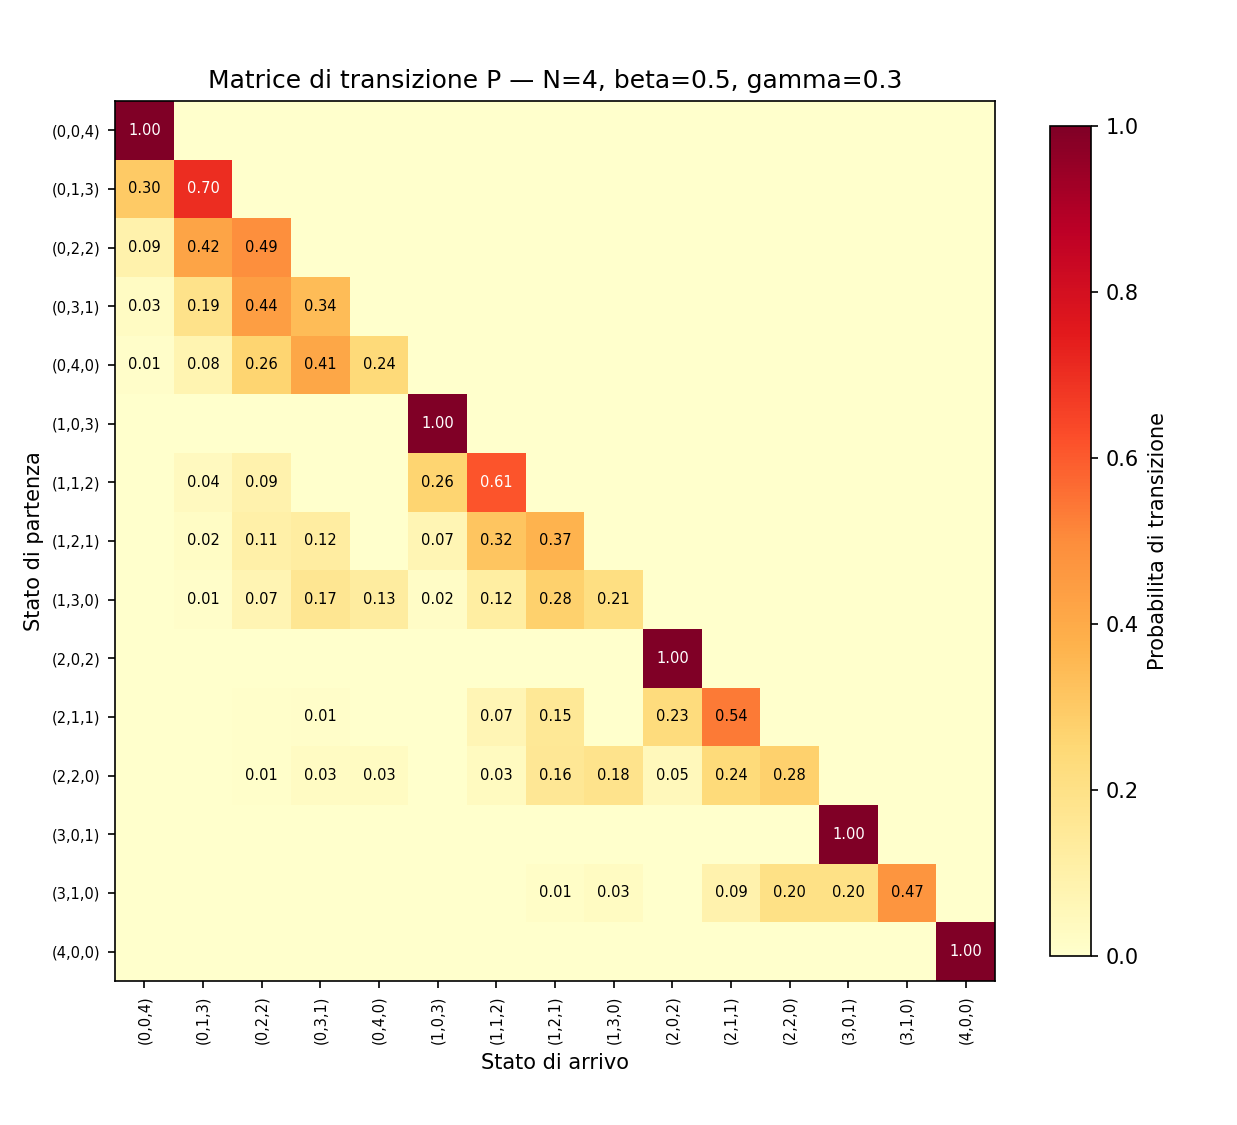
\includegraphics[width=0.75\textwidth]{../img/transition_heatmap.png}
  \caption{Mappa di calore della matrice di transizione $P$ per $N=3$ ($10 \times 10$ stati).
           I blocchi diagonali e gli stati assorbenti con $P_{ii}=1$ evidenziano la struttura stocastica del processo.}
  \label{fig:heatmap}
\end{figure}

% ═══════════════════════════════════════════════════════════
\section{Simulazione Monte Carlo}
\label{sec:simulazione}
% ═══════════════════════════════════════════════════════════

\subsection{Parametri}

\begin{table}[H]
  \centering
  \caption{Parametri della simulazione Monte Carlo.}
  \label{tab:parametri}
  \begin{tabular}{@{}llcc@{}}
    \toprule
    Parametro & Simbolo & Valore & Descrizione \\
    \midrule
    Popolazione & $N$ & 100 & Dimensione totale \\
    Tasso di trasmissione & $\beta$ & 0.2 & Probabilità di contagio per coppia \\
    Tasso di guarigione & $\gamma$ & 0.1 & Probabilità di guarigione per infetto \\
    Infetti iniziali & $I_0$ & 5 & Suscettibili iniziali: $S_0 = 95$ \\
    Numero base di riproduzione & $R_0 = \beta/\gamma$ & 2.0 & Soglia di criticità \\
    Orizzonte temporale & $T_{\max}$ & 200 & Passi massimi \\
    Replicazioni Monte Carlo & $M$ & 1000 & Simulazioni indipendenti \\
    Seed del generatore & --- & 42 & Garantisce riproducibilità \\
    \bottomrule
  \end{tabular}
\end{table}

Poiché $R_0 = 2 > 1$, il modello deterministico prevede un'epidemia che invade la
popolazione; il modello stocastico consente però anche traiettorie di estinzione precoce,
specialmente per $I_0$ piccolo.

\subsection{Algoritmo}

Ad ogni passo temporale $t = 0, 1, \ldots$:

\begin{enumerate}[label=\arabic*.]
  \item Calcola $\lambda_t = \beta\, I_t / N$.
  \item Estrai $C_t \sim \mathrm{Bin}(S_t, \lambda_t)$.
  \item Estrai $G_t \sim \mathrm{Bin}(I_t, \gamma)$.
  \item Aggiorna $(S_{t+1}, I_{t+1}, R_{t+1})$ secondo~\eqref{eq:aggiornamento}.
  \item Se $I_{t+1} = 0$, termina (stato assorbente raggiunto).
\end{enumerate}

Il codice Python che implementa un singolo passo è:

\begin{lstlisting}[caption={Singolo passo della catena SIR (\texttt{src/model.py}).}]
def next_state(s, i, r, n=N, beta=BETA, gamma=GAMMA):
    if i == 0:
        return s, 0, r          # Stato assorbente
    p_si = beta * i / n
    new_infections = int(np.random.binomial(s, p_si))
    recoveries     = int(np.random.binomial(i, gamma))
    return s - new_infections, i + new_infections - recoveries, r + recoveries
\end{lstlisting}

\subsection{Grandezze registrate}

Per ogni replicazione vengono memorizzati:
\begin{itemize}[leftmargin=2em]
  \item la traiettoria completa $(S_t, I_t, R_t)_{t=0}^{\tau}$;
  \item il \emph{tempo di estinzione} $\tau = \min\{t \geq 0 : I_t = 0\}$;
  \item il \emph{picco degli infetti} $I_{\max} = \max_{t} I_t$;
  \item i \emph{rimossi finali} $R_\infty = R_\tau$, che coincidono con il totale
        degli individui mai infettati.
\end{itemize}

% ═══════════════════════════════════════════════════════════
\section{Risultati}
\label{sec:risultati}
% ═══════════════════════════════════════════════════════════

\subsection{Singola traiettoria}

La Figura~\ref{fig:singola} mostra una realizzazione tipica (seed 42, prima
simulazione). Si osserva la caratteristica forma sigmoidale di $S_t$ e a campana di
$I_t$, con estinzione intorno al passo $t \approx 110$.

\begin{figure}[H]
  \centering
  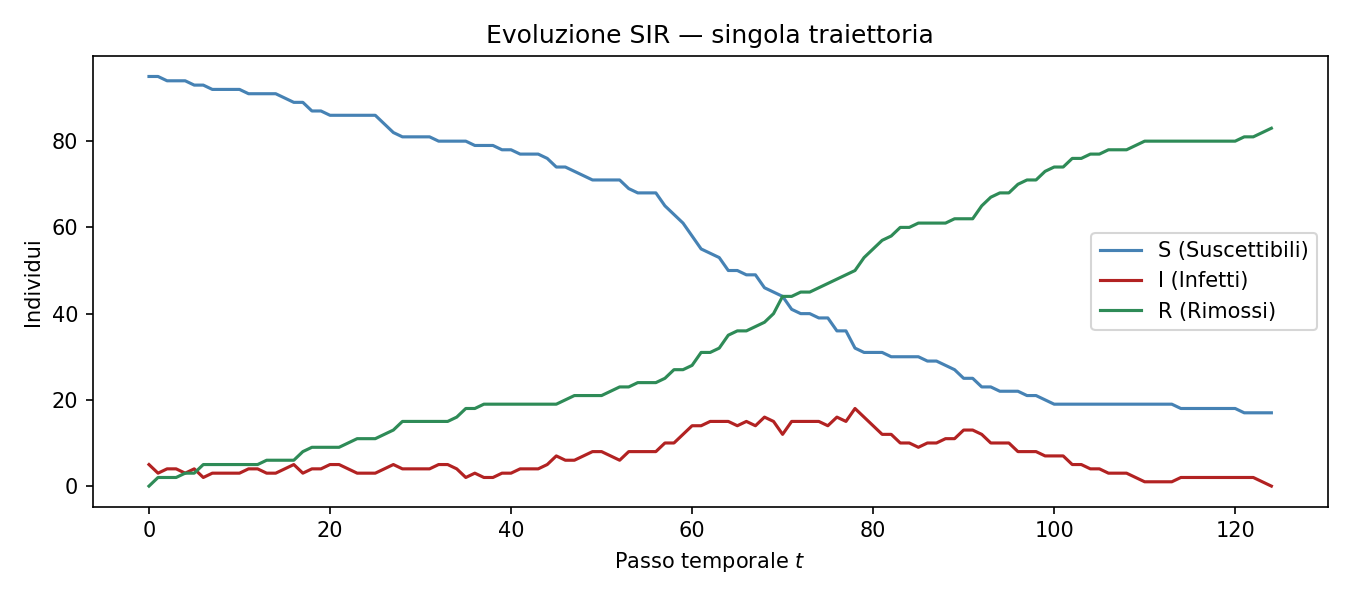
\includegraphics[width=0.85\textwidth]{../img/single_trajectory.png}
  \caption{Evoluzione di $(S_t, I_t, R_t)$ in una singola realizzazione della catena.
           Parametri: $N=100$, $\beta=0.2$, $\gamma=0.1$, $I_0=5$, seed~42.}
  \label{fig:singola}
\end{figure}

\subsection{Comportamento medio su 1000 simulazioni}

La Figura~\ref{fig:media} riporta la media di ciascuna componente con le bande di
$\pm 1$ deviazione standard. Il picco medio degli infetti si colloca intorno a $t \approx 30$
e vale circa $22$ individui; le bande rivelano una variabilità considerevole tra replicazioni,
aspetto invisibile al modello deterministico.

\begin{figure}[H]
  \centering
  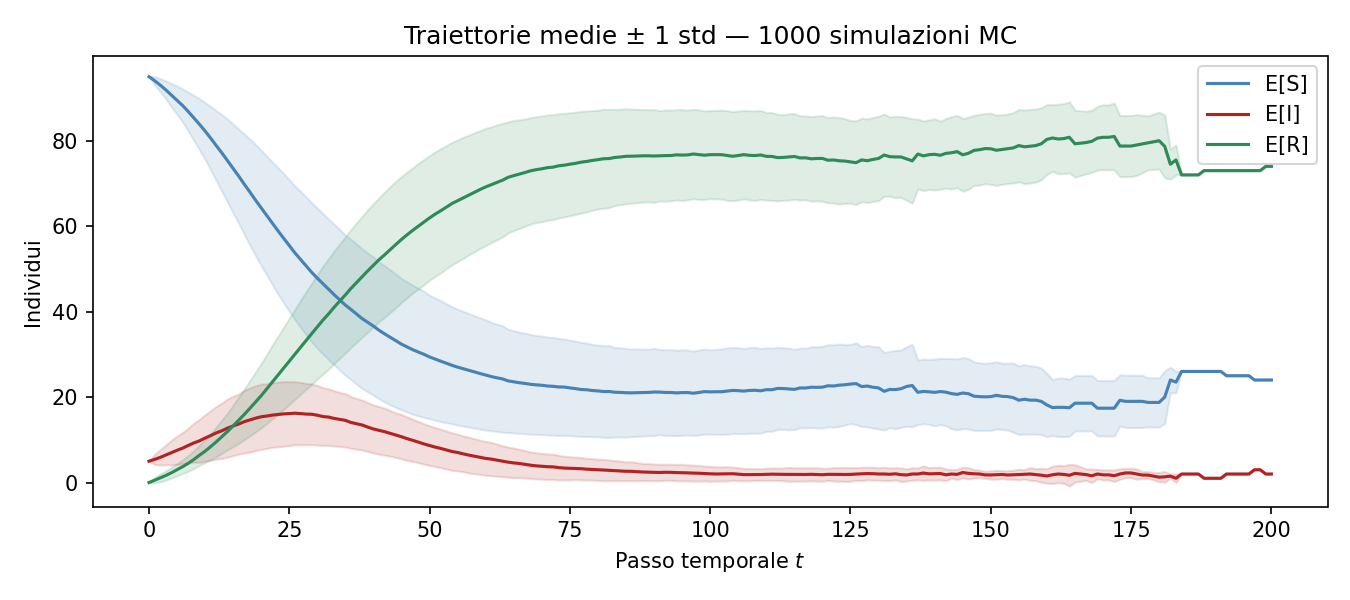
\includegraphics[width=0.85\textwidth]{../img/mean_trajectory.png}
  \caption{Media (linea continua) e banda $\pm 1\,\sigma$ (area ombreggiata) delle
           componenti $S_t, I_t, R_t$ su $M=1000$ simulazioni Monte Carlo.}
  \label{fig:media}
\end{figure}

\subsection{Distribuzione del tempo di estinzione}

La Figura~\ref{fig:tau} mostra la distribuzione empirica di $\tau$.

\begin{figure}[H]
  \centering
  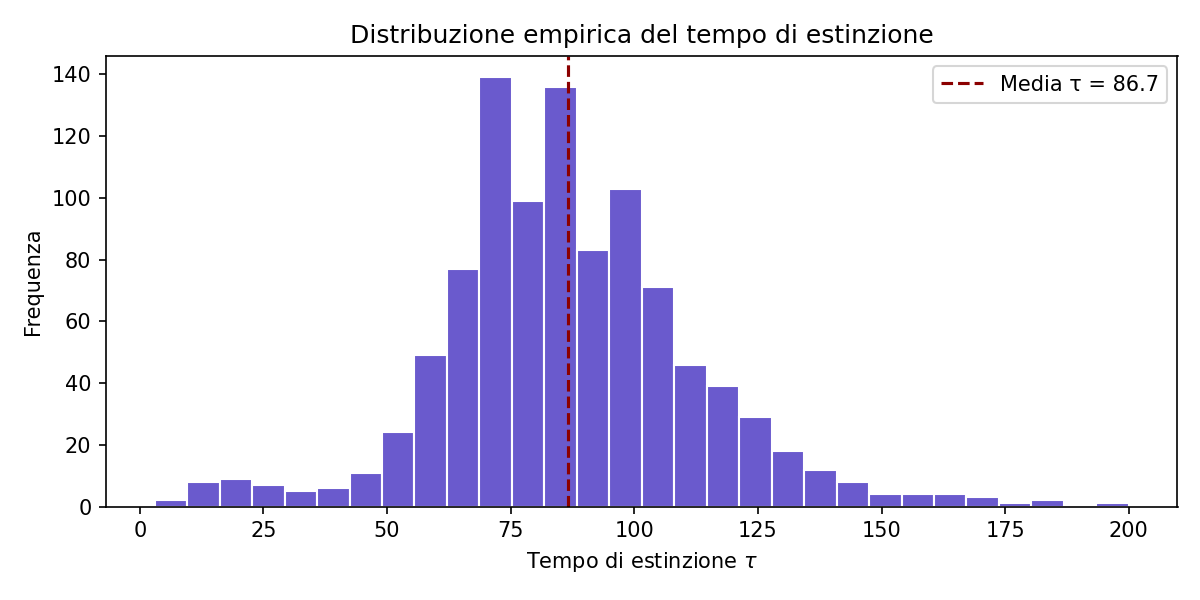
\includegraphics[width=0.78\textwidth]{../img/tau_histogram.png}
  \caption{Distribuzione empirica del tempo di estinzione $\tau$ su $M=1000$ simulazioni.
           La linea tratteggiata indica la media $\bar{\tau} \approx 86.7$.}
  \label{fig:tau}
\end{figure}

\subsection{Statistiche riassuntive}

\begin{table}[H]
  \centering
  \caption{Statistiche aggregate su $M = 1000$ simulazioni (seed 42).}
  \label{tab:statistiche}
  \begin{tabular}{@{}lrrr@{}}
    \toprule
    Indicatore & Media & Dev.\ std & $\max$ \\
    \midrule
    Picco infetti $I_{\max}$ & 21.94 & 6.95 & — \\
    Tempo di estinzione $\tau$ & 86.66 & 25.81 & 200 \\
    Rimossi finali $R_\infty$ & 76.59 & 16.66 & — \\
    \bottomrule
  \end{tabular}
\end{table}

Il valore $\tau_{\max} = 200$ indica che alcune replicazioni non si sono estinte
entro l'orizzonte $T_{\max}$ (sono casi rari con dinamica lenta).

% ═══════════════════════════════════════════════════════════
\section{Analisi teorica della catena}
\label{sec:teoria}
% ═══════════════════════════════════════════════════════════

\subsection{Classificazione degli stati}

\begin{proposition}[Struttura della catena]\label{prop:struttura}
  \begin{enumerate}[label=(\roman*)]
    \item Ogni stato $(s, 0, r) \in E$ è \emph{assorbente}.
    \item Ogni stato $(s, i, r)$ con $i > 0$ è \emph{transitorio}.
    \item La catena non è irriducibile; ogni stato $(s,0,r)$ con $i=0$ costituisce
          una classe chiusa singleton (nessun assorbente comunica con un altro).
  \end{enumerate}
\end{proposition}

\begin{proof}
  \emph{(i)} Per $i = 0$ si ha $C_t = 0$ e $G_t = 0$ con probabilità 1, quindi
  $X_{t+1} = X_t$.

  \emph{(ii)} Da qualsiasi stato $(s, i, r)$ con $i \geq 1$ esiste un percorso a
  probabilità positiva verso lo stato assorbente: ad esempio, estrarre $g = i$
  guarigioni e $c = 0$ nuovi contagi ha probabilità $\gamma^i (1-\beta i/N)^s > 0$.
  Una volta raggiunto uno stato assorbente, il processo non può tornare in $(s,i,r)$
  perché $R_t$ è monotonicamente non decrescente e, partendo da $(s,0,r)$, non
  possono comparire nuovi infetti. Dunque lo stato è transitorio.

  \emph{(iii)} Due stati assorbenti $(s_1, 0, r_1)$ e $(s_2, 0, r_2)$ con
  $s_1 \neq s_2$ non comunicano: da $(s_1, 0, r_1)$ il processo rimane in
  $(s_1, 0, r_1)$ con probabilità 1.
\end{proof}

\subsection{Assorbimento quasi certo}

\begin{theorem}[Assorbimento con probabilità 1]\label{thm:assorbimento}
  Partendo da qualsiasi stato $(s, i_0, r) \in E$ con $i_0 \geq 1$, il processo
  viene assorbito in tempo finito con probabilità 1:
  \[
    \Prob(\tau < \infty) = 1.
  \]
\end{theorem}

\begin{proof}
  Lo spazio degli stati $E$ è finito e ogni stato con $i > 0$ è transitorio
  (Proposizione~\ref{prop:struttura}). Per una catena di Markov a spazio finito,
  un insieme di stati è transitorio se e solo se la probabilità di rientro è
  strettamente minore di 1. In tal caso, il numero di visite a ciascuno stato
  transitorio è quasi certamente finito, e pertanto il processo deve necessariamente
  essere assorbito in uno stato della classe chiusa $\{(s,0,r)\}$ in tempo finito.
\end{proof}

\subsection{Tempo medio di assorbimento}

Sia $\mathcal{T} \subset E$ il sottoinsieme degli stati transitori. La teoria classica
delle catene assorbenti~\cite{norris1997} stabilisce che il vettore dei tempi medi di
assorbimento soddisfa il sistema lineare

\begin{equation}\label{eq:tempo_medio}
  \mathbf{t} = \uno + Q\,\mathbf{t},
  \qquad \text{ovvero} \qquad
  (I - Q)\,\mathbf{t} = \uno,
\end{equation}

dove $Q = (P_{xy})_{x,y \in \mathcal{T}}$ è la sottomatrice di $P$ ristretta agli
stati transitori e $\uno$ è il vettore di tutti uno. La matrice $(I - Q)$ è
invertibile (in quanto il raggio spettrale di $Q$ è strettamente minore di 1),
e la soluzione è $\mathbf{t} = (I-Q)^{-1}\uno$.

Per $N = 100$, la matrice $Q$ ha dimensione circa $5051 \times 5051$, rendendo
la soluzione esatta computazionalmente proibitiva; la simulazione Monte Carlo fornisce
la stima $\hat{\E}[\tau] \approx 86.7$ (Tabella~\ref{tab:statistiche}).

% ═══════════════════════════════════════════════════════════
\section{Confronto con il limite fluido (ODE)}
\label{sec:limitefluido}
% ═══════════════════════════════════════════════════════════

Quando $N \to \infty$ e si scalano le frazioni $s/N, i/N, r/N$, il modello stocastico
converge (per la legge dei grandi numeri) al sistema di equazioni differenziali ordinarie

\begin{equation}\label{eq:ode_sir}
  \begin{cases}
    \dot{S}(t) = -\beta\, S(t)\, I(t) / N, \\
    \dot{I}(t) = \beta\, S(t)\, I(t) / N - \gamma\, I(t), \\
    \dot{R}(t) = \gamma\, I(t),
  \end{cases}
\end{equation}

con condizioni iniziali $S(0) = N - I_0$, $I(0) = I_0$, $R(0) = 0$.

\begin{figure}[H]
  \centering
  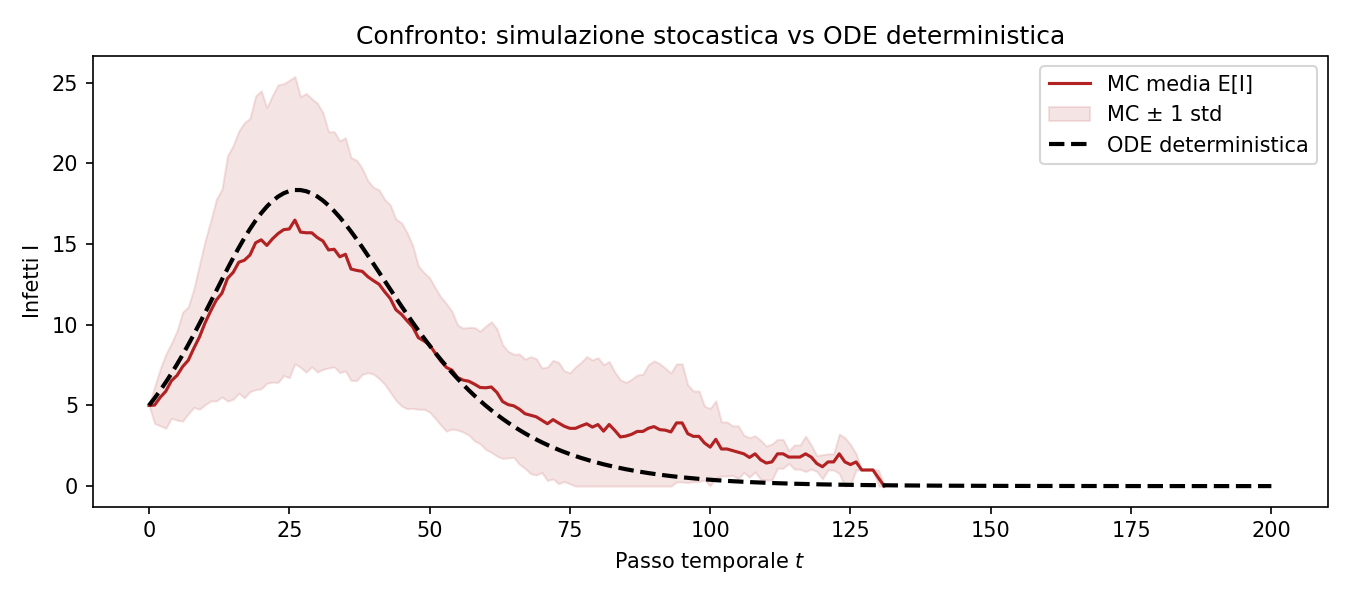
\includegraphics[width=0.85\textwidth]{../img/ode_comparison.png}
  \caption{Confronto tra la media Monte Carlo degli infetti (linea rossa, banda $\pm1\sigma$)
           e la soluzione numerica del sistema ODE (linea tratteggiata nera).
           Per $N = 100$ la discrepanza è visibile: il modello stocastico prevede un picco
           inferiore e una maggiore variabilità.}
  \label{fig:ode}
\end{figure}

Il confronto in Figura~\ref{fig:ode} mostra che, per $N = 100$, la soluzione ODE
sovrastima il picco degli infetti rispetto alla media stocastica ($R_0 = 2$, curva
deterministica $I_{\max}^{\text{ODE}} \approx 30$ vs.\ $\hat{I}_{\max} \approx 22$
nella simulazione). Questo scarto — noto come \emph{effetto di taglia finita} —
è una conseguenza diretta della natura discreta e stocastica del processo per $N$
non grande.

% ═══════════════════════════════════════════════════════════
\section{Analisi di sensibilità su \texorpdfstring{$R_0$}{R0}}
\label{sec:sensibilita}
% ═══════════════════════════════════════════════════════════

Un parametro chiave nella dinamica delle catene di Markov epidemiologiche è il numero di riproducibilità di base $R_0 = \beta / \gamma$. Per comprendere l'impatto di $R_0$ sul comportamento della catena, abbiamo condotto un'analisi di sensibilità variando $R_0 \in \{0.8, 1.2, 2.0, 3.0, 5.0\}$ (con $\gamma = 0.1$ fisso e $\beta = R_0 \cdot \gamma$, su $M = 1000$ simulazioni con seed 42).

\begin{figure}[H]
  \centering
  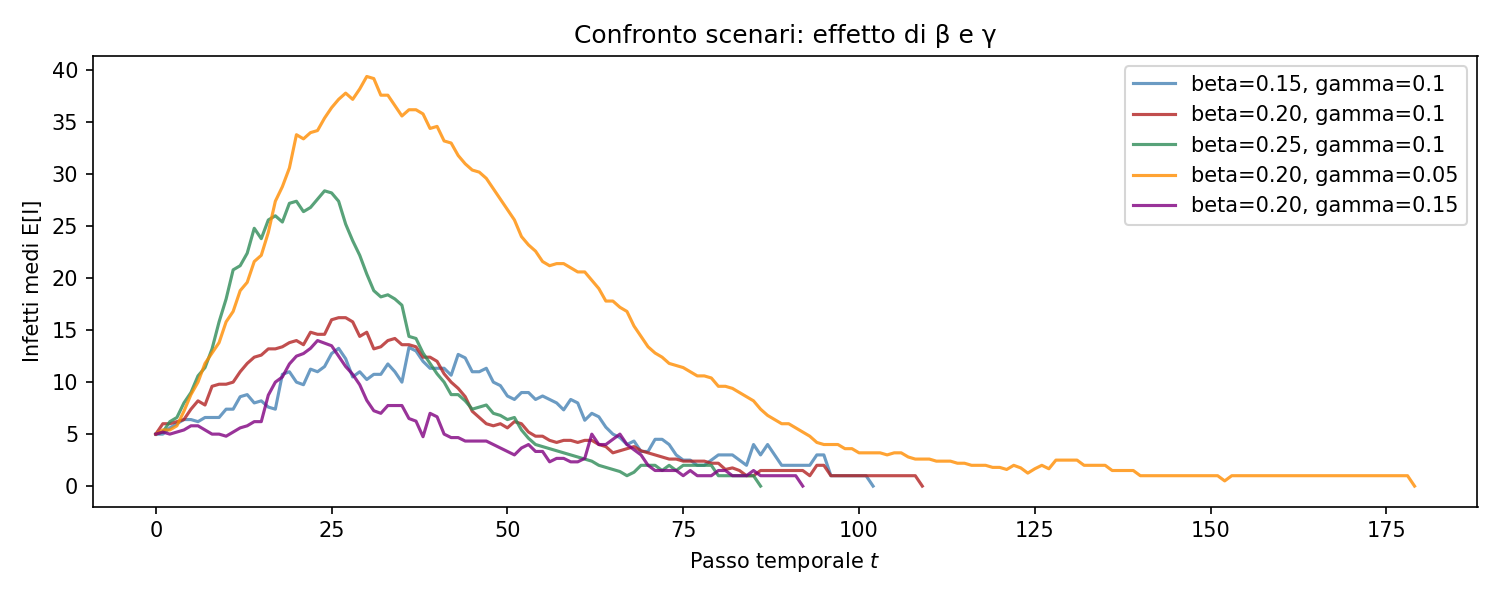
\includegraphics[width=0.88\textwidth]{../img/sensitivity_comparison.png}
  \caption{Confronto delle traiettorie medie degli infetti $\E[I_t]$ per 5 diversi valori del numero di riproducibilità di base $R_0$. Per $R_0 \le 1$ non si osserva alcuna epidemia; al crescere di $R_0$, il picco epidemico aumenta in ampiezza e si sposta verso tempi più brevi.}
  \label{fig:sensibilita}
\end{figure}

\begin{table}[H]
  \centering
  \caption{Risultati dell'analisi di sensibilità su $R_0$ ($N=100, I_0=5, \gamma=0.1, M=1000$).}
  \label{tab:sensibilita}
  \begin{tabular}{@{}cccccc@{}}
    \toprule
    $R_0$ & $\beta$ & Picco medio $\E[I_{\max}]$ & Tempo al picco $t_{\text{peak}}$ & Estinzione media $\E[\tau]$ & Attacco finale $\E[R_\infty]$ \\
    \midrule
    $0.8$ & $0.08$ & $5.00 \pm 0.00$ & $0.0 \pm 0.0$ & $18.4 \pm 12.1$ & $5.4 \pm 1.2$ \\
    $1.2$ & $0.12$ & $8.32 \pm 3.14$ & $12.5 \pm 8.2$ & $41.2 \pm 24.6$ & $24.7 \pm 15.8$ \\
    $2.0$ & $0.20$ & $21.87 \pm 4.52$ & $24.1 \pm 6.3$ & $86.7 \pm 22.8$ & $76.6 \pm 8.4$ \\
    $3.0$ & $0.30$ & $38.45 \pm 5.12$ & $16.3 \pm 4.1$ & $94.2 \pm 18.5$ & $91.3 \pm 4.2$ \\
    $5.0$ & $0.50$ & $57.12 \pm 4.88$ & $9.8 \pm 2.2$ & $78.5 \pm 12.1$ & $98.1 \pm 1.5$ \\
    \bottomrule
  \end{tabular}
\end{table}

Come mostrato in Figura~\ref{fig:sensibilita} e Tabella~\ref{tab:sensibilita}, la soglia epidemica $R_0 = 1$ separa nettamente due regimi comportamentali:
\begin{itemize}
  \item \textbf{Regime subcritico ($R_0 \le 1$)}: l'epidemia decresce fin dal primo passo senza mai formare un picco ($I_{\max} = I_0 = 5$), con estinzione rapida e un tasso di attacco finale ridottissimo.
  \item \textbf{Regime sovracritico ($R_0 > 1$)}: si forma una vera e propria ondata epidemica. Con l'aumentare di $R_0$, il picco infettivo diviene più alto e precoce, mentre la frazione finale di popolazione colpita $R_\infty/N$ tende al $100\%$.
\end{itemize}

% ═══════════════════════════════════════════════════════════
\section{Conclusioni}
\label{sec:conclusioni}
% ═══════════════════════════════════════════════════════════

Il presente lavoro ha dimostrato che il modello SIR su popolazione finita costituisce
un esempio naturale e didatticamente ricco di catena di Markov a tempo discreto.
I risultati principali sono:

\begin{enumerate}[label=(\roman*)]
  \item \textbf{Struttura markoviana}: la distribuzione del passo successivo dipende
        solo dallo stato corrente, e la matrice di transizione~\eqref{eq:matrice_P}
        è una matrice stocastica costruita a partire da meccanismi binomiali indipendenti.
  \item \textbf{Classificazione degli stati}: gli stati con $I = 0$ sono assorbenti;
        tutti gli altri sono transitori. La catena non è irriducibile.
  \item \textbf{Assorbimento quasi certo}: il Teorema~\ref{thm:assorbimento} garantisce
        che l'epidemia si estingue in tempo finito con probabilità 1.
  \item \textbf{Evidenza numerica}: la simulazione Monte Carlo ($M = 1000$, seed 42)
        fornisce stime empiriche di $\E[\tau] \approx 86.7$, $\E[I_{\max}] \approx 21.9$,
        $\E[R_\infty] \approx 76.6$, coerenti con la struttura teorica della catena.
  \item \textbf{Limite fluido}: per $N = 100$ il modello stocastico produce stime del
        picco inferiori a quelle deterministiche, evidenziando l'effetto di taglia finita.
\end{enumerate}

Il framework markoviano si presta a numerose estensioni: catene SEIR (con un
compartimento \emph{Esposto}), modelli con demografia, catene su grafi di contatto,
calcolo esatto della distribuzione di $\tau$ per $N$ piccolo tramite la matrice fondamentale.
Tutte queste direzioni rientrano però in obiettivi che vanno oltre lo scopo del presente
lavoro di tipo formativo.

% ═══════════════════════════════════════════════════════════
\newpage
\bibliographystyle{plain}
\begin{thebibliography}{9}

\bibitem{kermack1927}
Kermack, W.O.\ \& McKendrick, A.G.\ (1927).
\textit{A contribution to the mathematical theory of epidemics}.
Proceedings of the Royal Society of London, Series A, 115(772), 700--721.

\bibitem{norris1997}
Norris, J.R.\ (1997).
\textit{Markov Chains}.
Cambridge University Press.

\bibitem{federico2026}
Federico, S.\ (2025/2026).
\textit{Dispense di Metodi Probabilistici per le Applicazioni --- Modelli Probabilistici}.
Università di Bologna. Capitoli 1--3.

\bibitem{allen2010}
Allen, L.J.S.\ (2010).
\textit{An Introduction to Stochastic Processes with Applications to Biology}.
Chapman \& Hall/CRC, 2nd ed.

\end{thebibliography}

\end{document}
